Let a pair of homothetic, concentric, axis-aligned ellipses $\E$ and $\E_c$ have center at the origin. Let $a,b$ denote the semi-axes of $\E$. The semi-axes $a_c,b_c$ of $\E_c$ such that the pair admits a family of Poncelet N-periodics are be given by:

\[ a_c = a\cos\frac{\pi}{N},\;\;\;b_c = b\cos\frac{\pi}{N} \]

Since the family is an affine image of regular polygons interscribed in a concentric pair of circles, its area is invariant and given by:
\[A_N= N \sin \left( {\frac {2\pi}{N}} \right) \frac{ab}{2}\]

Referring to \cref{fig:homot_norm} (left):

\begin{lemma}
\label{lem:norm2}
Over Poncelet N-Periodics $\{p_1,\ldots p_n\}$ in the homothetic pair, the sum of squared norms $|p_k|^2$  is invariant and given by:

\[   \sum_{k=1}^N |p_k|^2=\frac{ N(a^2 + b^2)}{2}
	\]
\end{lemma}

\begin{figure}
    \centering
    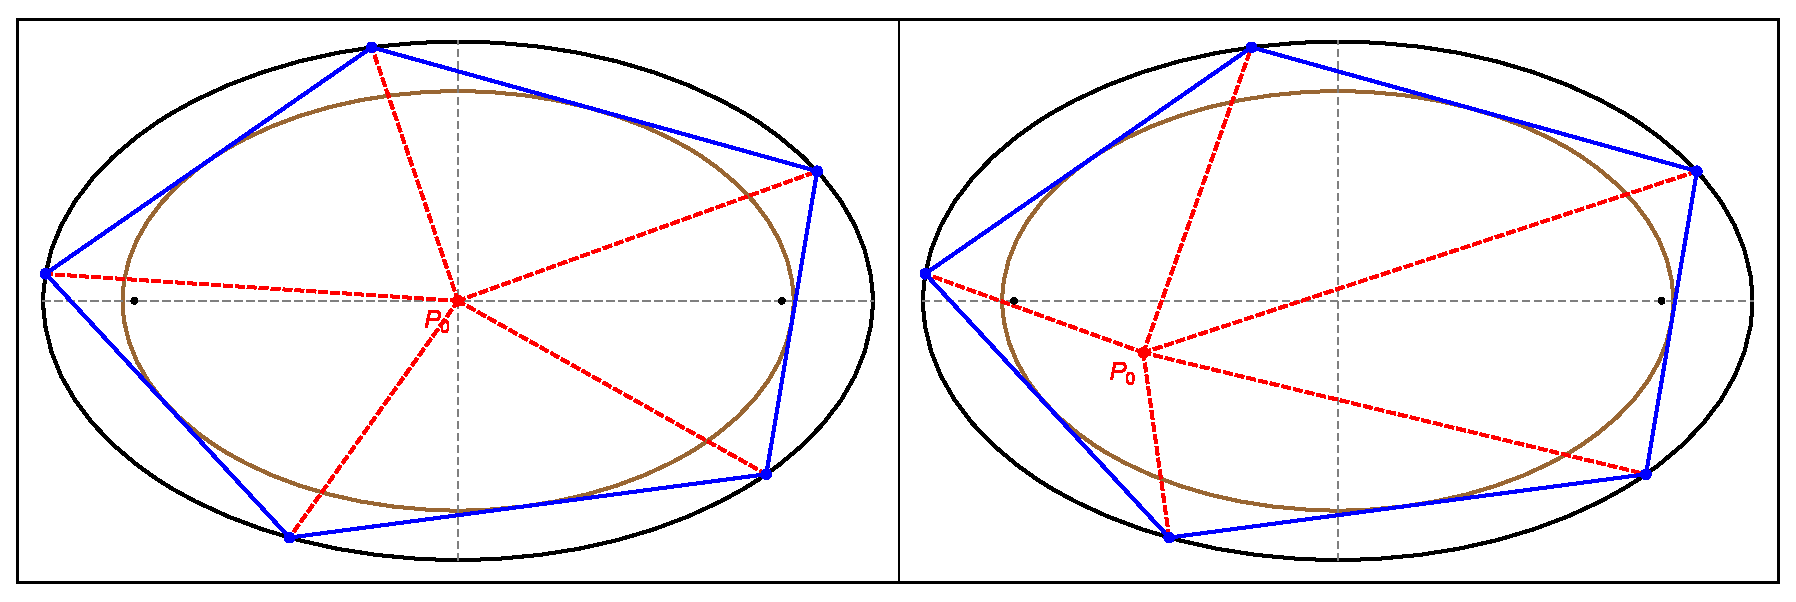
\includegraphics[width=\textwidth]{pics/0020_homot_norm.eps}
    \caption{\textbf{Left:} \cref{lem:norm2} states that the sum of squared norms of the vertices with respect to the center is invariant. \textbf{Right:} \cref{cor:p0} states that in fact the squared norms of vertices with respect to any point $P_0$ is invariant. \href{https://youtu.be/2PdsC3CcqaE}{Video}}.
    \label{fig:homot_norm}
\end{figure}

\noindent The proof below was kindly contributed by Sergei Tabachnikov
\cite{sergei2020-private-sidelengths}.

\begin{proof}
For the sake of the argument, we first consider the $N=3$ case. Define $v(\alpha)=(\cos \alpha, \sin \alpha)$ and a matrix $A$ which takes concentric circles to homothetic ellipses. Then $|Av(\alpha)|^2$ is a trigonometric polynomial of degree 2, and we average it over $\mathbb{Z}_3$ by adding $2\pi/3$ and $4\pi/3$ to $\alpha$. The result is independent of $\alpha$, as needed. Extending it to all $N$, note that a trigonometric polynomial of degree 2 averages to a constant over the action of $\mathbb{Z}_N$. The explicit expression was obtained via the the vertex parametrization below and CAS simplification.

%Let $P_1(t)=(x_1,y_1)=(a\cos{t},b\sin{t})$. Then $P_{k+1}=(x_{k+1},y_{k+1})$, $k=0...(N-1)$ are given by:

%\[ P_{k+1}=\left[a\cos \left( {\frac {2\,\pi\,k+tN}{N}} \right) ,b\sin \left( {\frac {2\,\pi\,k+tN}{N}} \right) \right]\]
\end{proof}

\begin{proposition}
\label{prop:sqr_si}
Over Poncelet N-Periodics in the homothetic pair, the sum of squared sidelengths $L_{2,N}$ is invariant. It is given by:

\[ L_{2,N}= \sum_{k=1}^N L_k^2=N \left[ 1-\cos \left(  {\frac {2\pi}{N}} \right)  \right]  \left(
{a}^{2}+{b}^{2} \right) 
	\]
\end{proposition}

\begin{proof}
The sidelengths are expressed by trigonometric polynomials of degree 2. So the proof is analogous to that of   \Cref{lem:norm2}.
\end{proof}
\noindent Referring to \cref{fig:brocard-n3}, recall the Brocard angle $\omega$ of a triangle is given by $\cot\omega=L_{2,3}/(4A_3)$ \cite[Brocard Angle]{mw}. Then:

\begin{corollary}
The family of 3-periodics in the homothetic pair conserves Brocard angle $\omega$.    
\end{corollary}

Note: a well-known identity is that $\cot\omega=\cot\theta_1+\cot\theta_2+\cot\theta_3$. \cref{th:cot} is statement that this sum generalizes for $N>3$. 

%\begin{corollary}
%	\[ 4\left(1-\cos\left(\frac{2\pi}{n}\right) \right)A_n Cot_n+ n\cos\left(\frac{2\pi}{n}\right) L_n=0\]
%\end{corollary}

Referring to \cref{fig:homot_norm}, the sum of squared distances from vertices to a fixed point $p_0$ is also invariant, owing to the same trigonometric polynomial argument:

\begin{corollary}
\[   \sum_{k=1}^N |p_k-p_0|^2=\frac{ N(a^2 + b^2)}{2} + N |p_0|^2
\]
\label{cor:p0}
\end{corollary}




